\exercise{5\textbar 1}{Outsourcing}

\textbf{Aufgabe:}  
Als Manager stehen Sie vor der Frage, ob Sie die bisher in Ihrem Unternehmen angesiedelte Druckerei schließen und die anfallenden Druckarbeiten extern ausführen lassen sollen.

\textbf{Fragestellung:}  
Von welchen Faktoren wird Ihre Entscheidung abhängen?

\solution{
\textbf{Lösung:}

\begin{itemize}
    \item Die Neue Institutionenökonomie lehrt, dass die Transaktionskosten die zentrale Determinante für solche organisatorischen Fragen darstellen.
    \item Ob Sie sich für das Outsourcing entscheiden oder nicht, hängt also davon ab, wie hoch Sie die Transaktionskosten bei den alternativen Lösungen einschätzen.
    \item Bei der Alternative \textbf{"Hierarchie"} (d. h. dem Beibehalten der hauseigenen Druckerei) sind die Transaktionskosten des Aushandelns der Verträge relativ gering.
    \begin{itemize}
        \item Es reicht, einen oder mehrere Arbeitsverträge mit den Arbeitnehmern in der Druckerei abzuschließen, die in der Regel eine längerfristige Laufzeit aufweisen.
    \end{itemize}
    \item Bei der Alternative \textbf{"Markt"} (d. h. dem externen Ausführen von Druckarbeiten) muss für jeden Auftrag ein neuer Vertrag abgeschlossen werden, was mit höheren Transaktionskosten des Vertragsschließens verbunden ist.
    \begin{itemize}
        \item Zu den Transaktionskosten zählen aber auch die Kosten der Überwachung der Leistungserbringung.
        \item Bei der externen Lösung kann durch den Vergleich mit unterschiedlichen Anbietern relativ einfach ermittelt werden, ob man die optimale Lösung gefunden hat.
    \end{itemize}
    \item Bei der hauseigenen Druckerei ist ein solcher Vergleich sehr viel schwieriger, sodass eine stärkere interne Überwachung erforderlich ist.
    \item Für die definitive Entscheidung kommt es neben dem Vergleich dieser Kostenkomponenten auch noch auf die sozialpolitischen Regeln eines Landes an.
\end{itemize}

\note{Hinweis:} Diese werden in Aufgabe 5\textbar 2 noch ausführlicher diskutiert.
}
\exercise{5\textbar 2}{Scheinselbstständigkeit}

\textbf{Aufgabe:}  
Zur Finanzierung der deutschen Einheit wurde in den 1990er-Jahren das System der sozialen Sicherungssysteme missbraucht.

\begin{itemize}
    \item Mit den Sozialabgaben wurden also teilweise verdeckte Steuern erhoben.
    \item Gleichzeitig konnte man in dieser Phase beobachten, dass die Anzahl der „Scheinselbstständigen“ deutlich anstieg.
    \item Dabei handelt es sich um Beschäftigte, die formal als Selbstständige Tätigkeiten wahrnehmen, die bisher in der Form eines Arbeitsvertrags organisiert waren.
\end{itemize}

\textbf{Aufgabe:} Erklären Sie diese Entwicklung.  
\textit{Hinweis:} Berücksichtigen Sie die Transaktionskosten einer arbeitsteiligen Wirtschaft.

\solution{

\begin{itemize}
    \item Dem Mikrozensus des Statistischen Bundesamts kann man eindrucksvolle Veränderungen in der Struktur der Beschäftigung entnehmen.
    \item Wie das Schaubild verdeutlicht, ist die Zahl der Vollzeit-Beschäftigten um 11 \% zurückgegangen, während die Teilzeitarbeit um 44 \% gestiegen ist.
    \item Auch die Zahl der Selbstständigen ist um 27 \% gestiegen, die der Selbstständigen ohne Mitarbeiter (d.h. Vorformen der „Ich-AG“) sogar um 32 \%.
    \item Diese Entwicklung ist wesentlich auf die Veränderungen in den Transaktionskosten zurückzuführen:
    \begin{itemize}
        \item Die Belastung des Vollzeitarbeitsplatzes durch steigende Sozialabgaben hat die Transaktionskosten dieser Form der Arbeitsteilung massiv erhöht.
        \item Deshalb ist der Markt auf Organisationsformen ausgewichen, die wie die Schein-Selbstständigkeit von dieser verdeckten Form der Besteuerung nicht betroffen wurden.
    \end{itemize}
\end{itemize}

\vspace{0.5cm}
\textbf{Grafik:} Veränderung ausgewählter Erwerbsformen (Mikrozensus 2001)  
\begin{figure}[H]
    \centering
    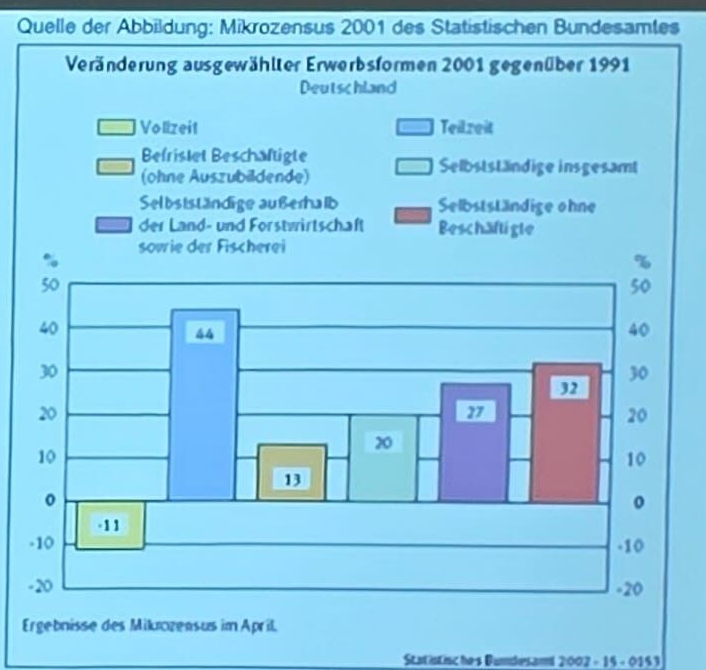
\includegraphics[width=0.8\textwidth]{figures/5_2.png} % Platzhalter für die Grafik
    \caption{Quelle: Statistisches Bundesamt, Mikrozensus 2001}
    \label{fig:scheinselbststaendigkeit}
\end{figure}
}
\exercise{5\textbar 3}{„Small is beautiful“}

\textbf{Aufgabe:}  
In Deutschland gibt es viele kleine und mittlere Unternehmen, die auf den Weltmärkten sehr erfolgreich sind.  
Wie kann man erklären, dass Großunternehmen nicht grundsätzlich wettbewerbsfähiger sind als kleine Unternehmen?

\solution{

\begin{itemize}
    \item Ein \textbf{großes Unternehmen} hat viele \textbf{Vorteile} gegenüber einem kleinen:
    \begin{itemize}
        \item So können die Durchschnittskosten bei einer steigenden Produktionsmenge sinken (\textit{„steigende Skalenerträge“}).
        \item Auch verfügt ein Großunternehmen oft über eine \textbf{bessere Verhandlungsposition} bei Abnehmern wie auch bei Lieferanten.
    \end{itemize}
    
    \item Der \textbf{Nachteil} eines großen Unternehmens besteht jedoch darin, dass dort die \textbf{Arbeitsteilung überwiegend nach dem Prinzip der Hierarchie} organisiert ist.
    \begin{itemize}
        \item Dabei stellt sich das Problem, dass hohe Transaktionskosten durch das \textit{„Principal-Agent“-Problem} geschaffen werden, die man auch als \textit{„Motivation Costs“} bezeichnet.
    \end{itemize}
    
    \item Das kleine Unternehmen führt sehr viele Transaktionen nach dem \textbf{Prinzip des Marktes} durch, womit solche Kosten vermieden werden können.
    
    \item Die Problematik einer zu weitgehenden Unternehmenskonzentration wurde besonders deutlich in den Ländern Osteuropas und der ehemaligen Sowjetunion, in denen die Wirtschaft bis 1990 nach dem Prinzip eines einzigen Großunternehmens organisiert war.
\end{itemize}
}

